\section{\textcolor{unibablueI}{Time Table}}
%
\newcommand{\daywidth}{24mm}
\newcommand{\daytextwidth}{21mm}
%
\newcommand{\hourseparation}{3mm}
%
\begin{tikzpicture}[yscale=-0.1, xscale=0.1, node distance=1mm,inner sep = 0pt, outer sep = 0pt]
%
% Style for Days
\tikzstyle{day}=[draw, white, rectangle,  minimum height=5mm, minimum width=\daywidth, fill=unibablueI,anchor=north west, align=center, font=\small]
% Style for hours
\tikzstyle{hour}=[draw, rectangle, minimum height=5mm, minimum width=8mm, fill=unibagrayIV, anchor=north west, align=center, font=\scriptsize]
%
\tikzstyle{default}=[anchor=north west,draw=red]
%
% Styles for events
% Duration of sequences
\tikzstyle{hours}=[rectangle,draw, minimum width=\daywidth, text width=\daytextwidth, anchor=north west, align=center, font=\footnotesize]
\tikzstyle{hhours}=[rectangle,draw, minimum width=.5*\daywidth-1.5mm, text width=.5*\daytextwidth-1.5mm, anchor=north west, align=center, font=\footnotesize]
%
\tikzset{grid/.style={gray,very thin,opacity=1}}
%
%\node[default] at (-7,-12) {
%        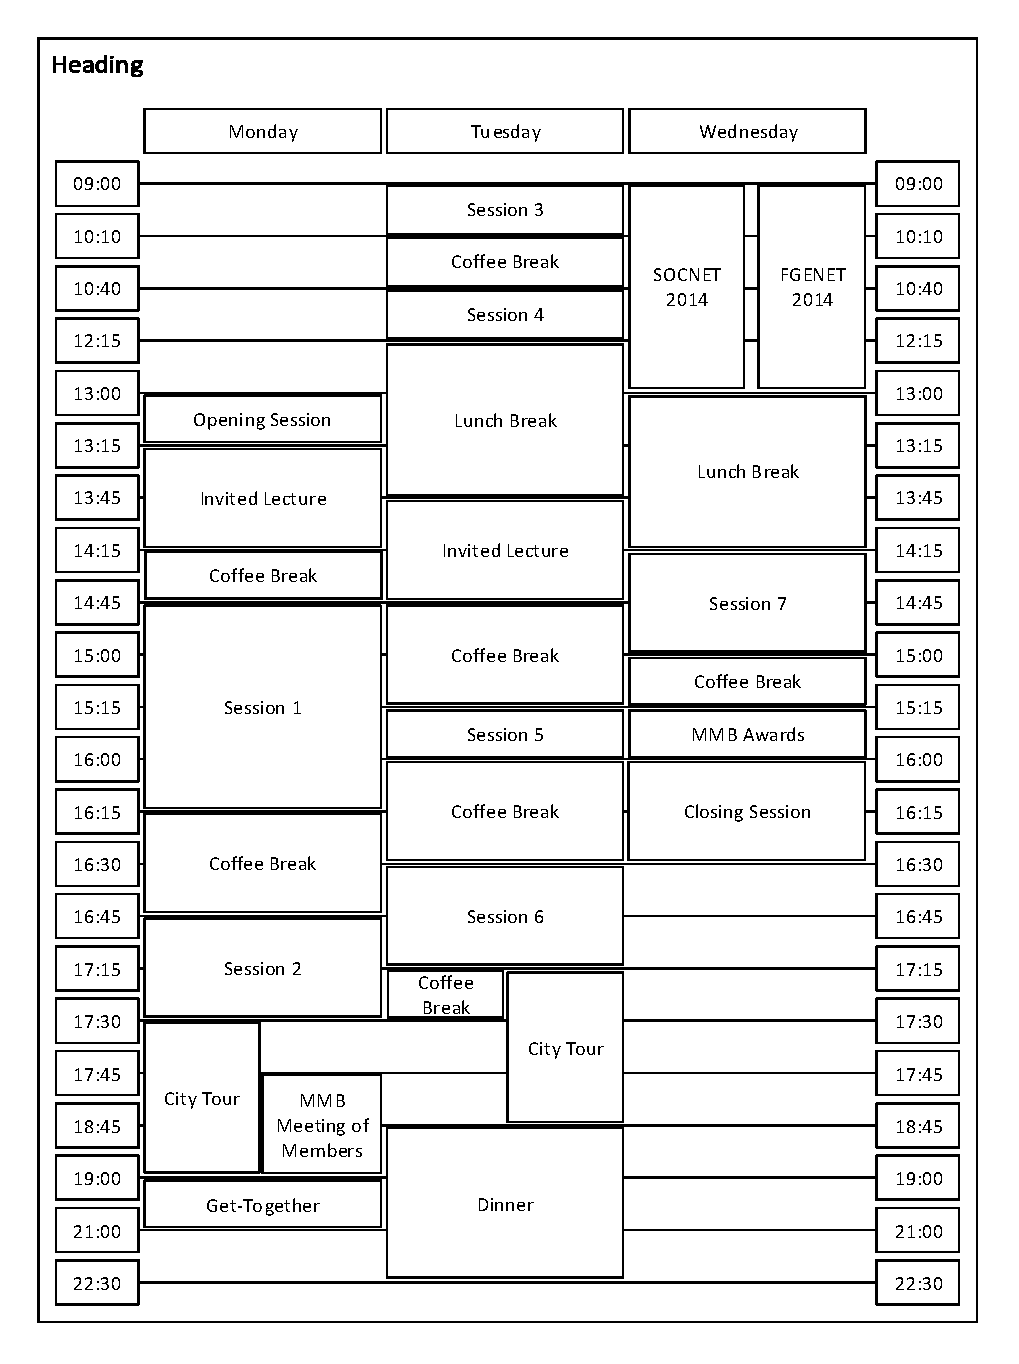
\includegraphics[width=2cm+\textwidth]{images/timetable.pdf}
%    };
%   
%\draw[grid] (0,0) grid (10*\textwidth,10*\textheight);
%
\node[day] (so) at (9,0) {SOCNET};
\node[day] (fg) [right = of so] {FGENET};
\node[day] (wo) [right = of fg] {WoNeCa};
%
\node[hour] (0900) at (0,7) {09:00};
\node[hour] (1000) [below = \hourseparation of 0900] {10:00};
\node[hour] (1020) [below = \hourseparation of 1000] {10:20};
%\node[hour] (1215) [below = \hourseparation of 1040] {12:15};
%\node[hour] (1300) [below = \hourseparation of 1215] {13:00};
%\node[hour] (1315) [below = \hourseparation of 1300] {13:15};
%\node[hour] (1345) [below = \hourseparation of 1315] {13:45};
%\node[hour] (1415) [below = \hourseparation of 1345] {14:15};
%\node[hour] (1445) [below = \hourseparation of 1415] {14:45};
%\node[hour] (1500) [below = \hourseparation of 1445] {15:00};
%\node[hour] (1515) [below = \hourseparation of 1500] {15:15};
%\node[hour] (1600) [below = \hourseparation of 1515] {16:00};
%\node[hour] (1615) [below = \hourseparation of 1600] {16:15};
%\node[hour] (1630) [below = \hourseparation of 1615] {16:30};
%\node[hour] (1645) [below = \hourseparation of 1630] {16:45};
%\node[hour] (1715) [below = \hourseparation of 1645] {17:15};
%\node[hour] (1730) [below = \hourseparation of 1715] {17:30};
%\node[hour] (1745) [below = \hourseparation of 1730] {17:45};
%\node[hour] (1845) [below = \hourseparation of 1745] {18:45};
%\node[hour] (1900) [below = \hourseparation of 1845] {19:00};
%\node[hour] (2100) [below = \hourseparation of 1900] {21:00};
%\node[hour] (2230) [below = \hourseparation of 2100] {22:30};
%
% SOCNET
%\node[hours, minimum height = 7mm, fill=white] (os) at($(1300.west)+(mo.north west)+(0,.5)$) {Opening Session};
%\node[hours, minimum height = 15mm, fill=unibayellowV] (il1) [below = of os] {Invited Lecture\\ S{\o}ren Asmussen};
%\node[hours, minimum height = 7mm, fill=white] (cb1) [below = of il1] {Coffee Break};
%\node[hours, minimum height = 31mm, fill=unibablueV] (s1) [below = of cb1] {Session 1};
%\node[hours, minimum height = 15mm, fill=white] (cb2) [below = of s1] {Coffee Break};
%\node[hours, minimum height = 15mm, fill=unibablueV] (s2) [below = of cb2] {Session 2};

%
% FGENET
\node[hours, minimum height = 7mm, fill=unibablueV] (fgs1) at($(0900.west)+(fg.north west)+(0,.5)$) {Session 1};
\node[hours, minimum height = 7mm, fill=white] (fgcb1) [below = of fgs1] {Coffee Break};
%\node[hours, minimum height = 7mm, fill=unibablueV] (s4) [below = of cb3] {Session 4};
%\node[hours, minimum height = 23mm, fill=white] (lb1) [below = of s4] {Lunch Break};
%\node[hours, minimum height = 15mm, fill=unibayellowV] (il2) [below = of lb1] {Invited Lecture\\ James Roberts};
%\node[hours, minimum height = 15mm, fill=white] (cb4) [below = of il2] {Coffee Break};
%\node[hours, minimum height = 7mm, fill=unibablueV] (s5) [below = of cb4] {Session 5};
%\node[hours, minimum height = 15mm, fill=white] (cb5) [below = of s5] {Coffee Break};
%\node[hours, minimum height = 15mm, fill=unibagrayV] (s6) [below = of cb5] {Session 6};

% WoNeCa
%\node[hours, minimum height = 31mm, fill=unibagreenV] (so) at($(0900.west)+(we.north west)+(0,.5)$) {\footnotesize Workshops\\[3ex] \footnotesize SOCNET\\[1ex] \footnotesize FGENET\\[1ex] \footnotesize WoNeCa (-- 16:00)};
%\node[hours, minimum height = 23mm, fill=white] (lb2) at($(1300.west)+(we.north west)+(0,.5)$) {Lunch Break};
%\node[hours, minimum height = 15mm, fill=unibablueV] (s7) [below = of lb2] {Session 7};
%\node[hours, minimum height = 7mm, fill=white] (cb7) [below = of s7] {Coffee Break};
%\node[hours, minimum height = 7mm, fill=unibaredV] (ma) [below = of cb7] {MMB Awards};
%\node[hours, minimum height = 15mm, fill=white] (cs) [below = of ma] {Closing Session};
\end{tikzpicture}
\enlargethispage{3ex}